\begin{IEEEkeywords}
UAV Localization, GNSS-denied Navigation, Image Registration, Feature Matching, Affine Transformation, RANSAC, SIFT
\end{IEEEkeywords}

\section{Introduction}

\subsection{Problem Context}
Visual Unmanned Aerial Vehicle (UAV) localization enables autonomous flight by calculating absolute geographic coordinates solely from optical sensors. This involves matching the UAV's real-time images against georeferenced satellite maps.

\begin{figure}[htbp]
    \centering
    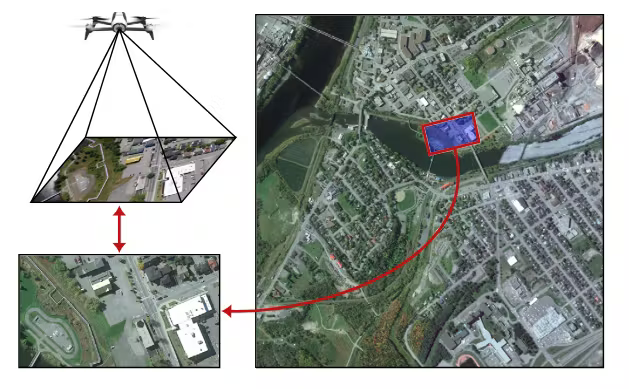
\includegraphics[width=1\columnwidth]{figs/image_to_map_localization.png}
    \caption{Matching the UAV camera feed to a reference satellite map \cite{b1}.}
    \label{fig:image_to_map}
\end{figure}

These systems are critical in modern warfare, where Electronic Warfare (EW) makes Global Navigation Satellite Systems (GNSS) highly vulnerable. Vision-based localization offers a passive, unjammable alternative, allowing UAVs to compute coordinates from onboard visual data and navigate GNSS-denied environments.

This project develops an automated vision-based positioning system for UAVs.
